\documentclass{article}
  \usepackage[total={18cm,21cm},top=2cm, left=2cm]{geometry}
  %Paquetes adicionales
  \usepackage{latexsym,amsmath,amssymb,amsfonts}
  \usepackage[latin1]{inputenc}
  %\usepackage{txfonts}
  \usepackage[T1]{fontenc}\usepackage{ae,aecompl}
  \usepackage{graphicx}
\usepackage[usenames]{color}
\usepackage[spanish]{babel} % Idioma espa�ol
\usepackage{tcolorbox}
\usepackage{multirow}
\tcbuselibrary{theorems}
\usepackage{listings}
\lstset{moredelim=[is][\itshape]{|}{|}}
\usepackage{mathrsfs}
  %---------------comandos especiales-------------------------------
	
  %-----------------------------------------------------------------

\begin{document}
\begin{center}
{\sc Calculo diferencial e integral III} 
\end{center}
\noindent{\sc Angie Marchena  } \hfill   \\
\noindent{\sc Mercedes Rojas  } \hfill   \\
{\sc Rodolfo Mart�n } \hfill   \\
\begin{center}
{\sc Actividad programada 1 }\\
\end{center}

\section*{Pregunta 1}
\begin{enumerate}
\item[$a)$] Parametrizar la curva de la siguiente gr�fica.
\begin{center}
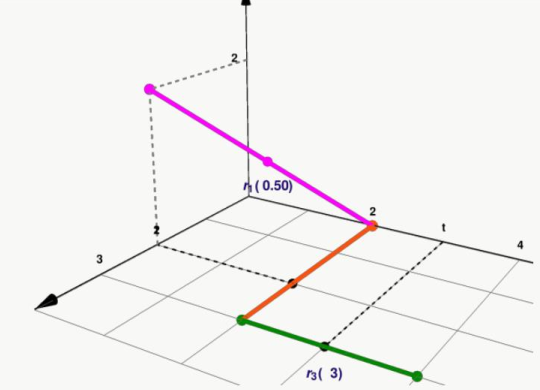
\includegraphics[scale=0.5]{p1}
\end{center}
Podemos obtener los puntos que est�n en cada segmento:\\


\begin{minipage}[t]{0.3\textwidth}
Para $r_1$: (2,0,2) y (0,2,0)
\end{minipage} \begin{minipage}[t]{0.3\textwidth}
Para $r_2$: (3,2,0) y (0,2,0)
\end{minipage}\begin{minipage}[t]{0.3\textwidth}
Para $r_3$: (3,2,0) y (3,4,0)
\end{minipage}
Con esto podemos realizar la parametrizacion mediante mediante la formula:

$$r(t) = P + t(Q-P)$$

Donde $P$ y $Q$ son puntos que est�n en el segmento de recta.

Procedemos con el calculo de los segmentos parametrizados.\\\\


\begin{minipage}[t]{0.3\textwidth}
Para $r_1$: (2,0,2) y (0,2,0)
\begin{align*}
&(0,2,0)-(2,0,2)=(-2,2,-2)\\
&r_1(t) = (2,0,2) + t(-2,2,-2)\\
&r_1(t) = (2-2t,2t,2-2t)
\end{align*}
$$\left\{\begin{matrix}
x =& 2-2t& \\ 
y =& 2t&t\in[0,1] \\ 
z =& 2-2t&
\end{matrix}\right.$$
\end{minipage} \begin{minipage}[t]{0.3\textwidth}
Para $r_2$: (0,2,0) y (3,2,0)
\begin{align*}
&(3,2,0)-(0,2,0)=(3,0,0)\\
&r_2(t) = (0,2,0) + t(3,0,0)\\
&r_2(t) = (3t,2,0)
\end{align*}
$$\left\{\begin{matrix}
x =& 3t& \\ 
y =& 2&t\in[0,1] \\ 
z =& 0&
\end{matrix}\right.$$
\end{minipage}\begin{minipage}[t]{0.3\textwidth}
Para $r_3$: (3,2,0) y (3,4,0)
\begin{align*}
&(3,4,0)-(3,2,0)=(0,2,0)\\
&r_3(t) = (3,2,0) + t(0,2,0)\\
&r_3(t) = (3,2+2t,0)
\end{align*}
$$\left\{\begin{matrix}
x =& 3& \\ 
y =& 2+2t&t\in[0,1] \\ 
z =& 0&
\end{matrix}\right.$$
\end{minipage}
\clearpage



\item[$b)$] Al realizar la grafica se puede ver que coinciden.
\begin{center}
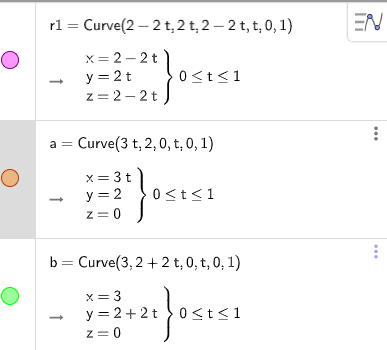
\includegraphics[scale=0.4]{p1c}\\
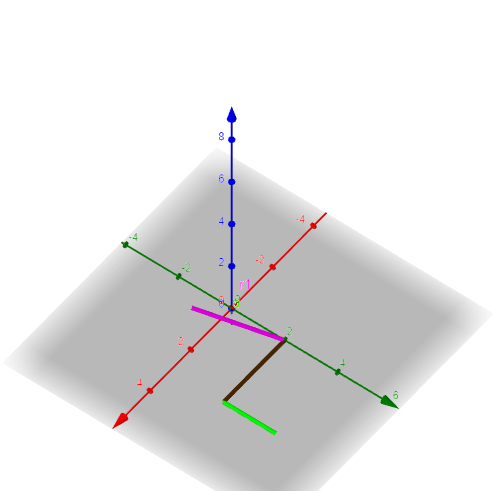
\includegraphics[scale=0.4]{p1b}
\end{center}
\end{enumerate}



\clearpage
\section*{Pregunta 2}
\begin{enumerate}
\item[$a)$] Graficar mediante GeoGebra las superficies:
\begin{align*}
&x^2+y^2=9\\
&z=x+y
\end{align*}
\begin{center}
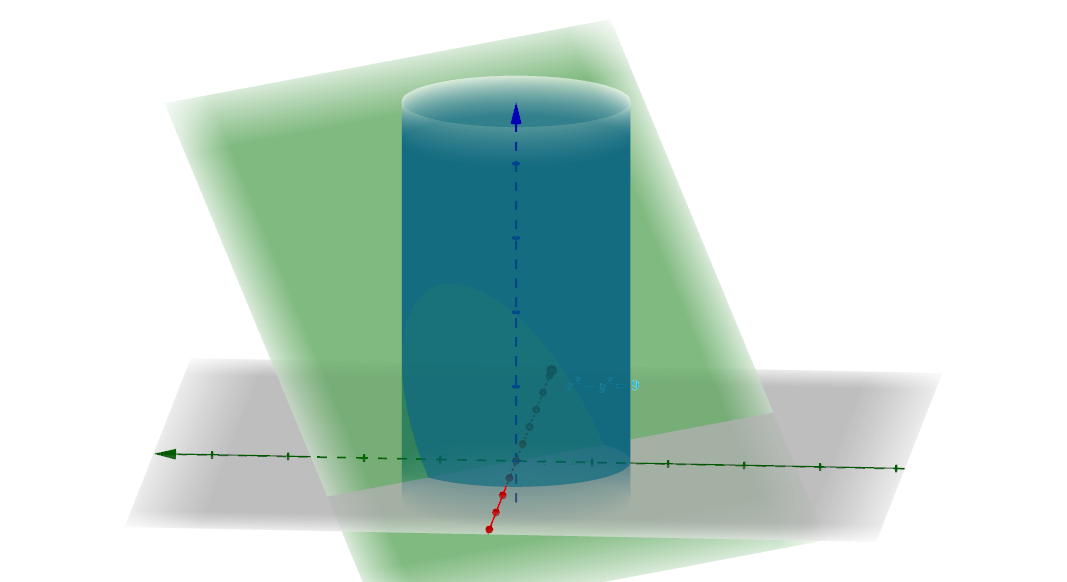
\includegraphics[scale=1]{p2a}
\end{center}
Se puede ver el plano  en color verde y el cilindro en color celeste.

\item[$b)$] La intersecci�n entre las dos superficies es una elipse.
\begin{center}
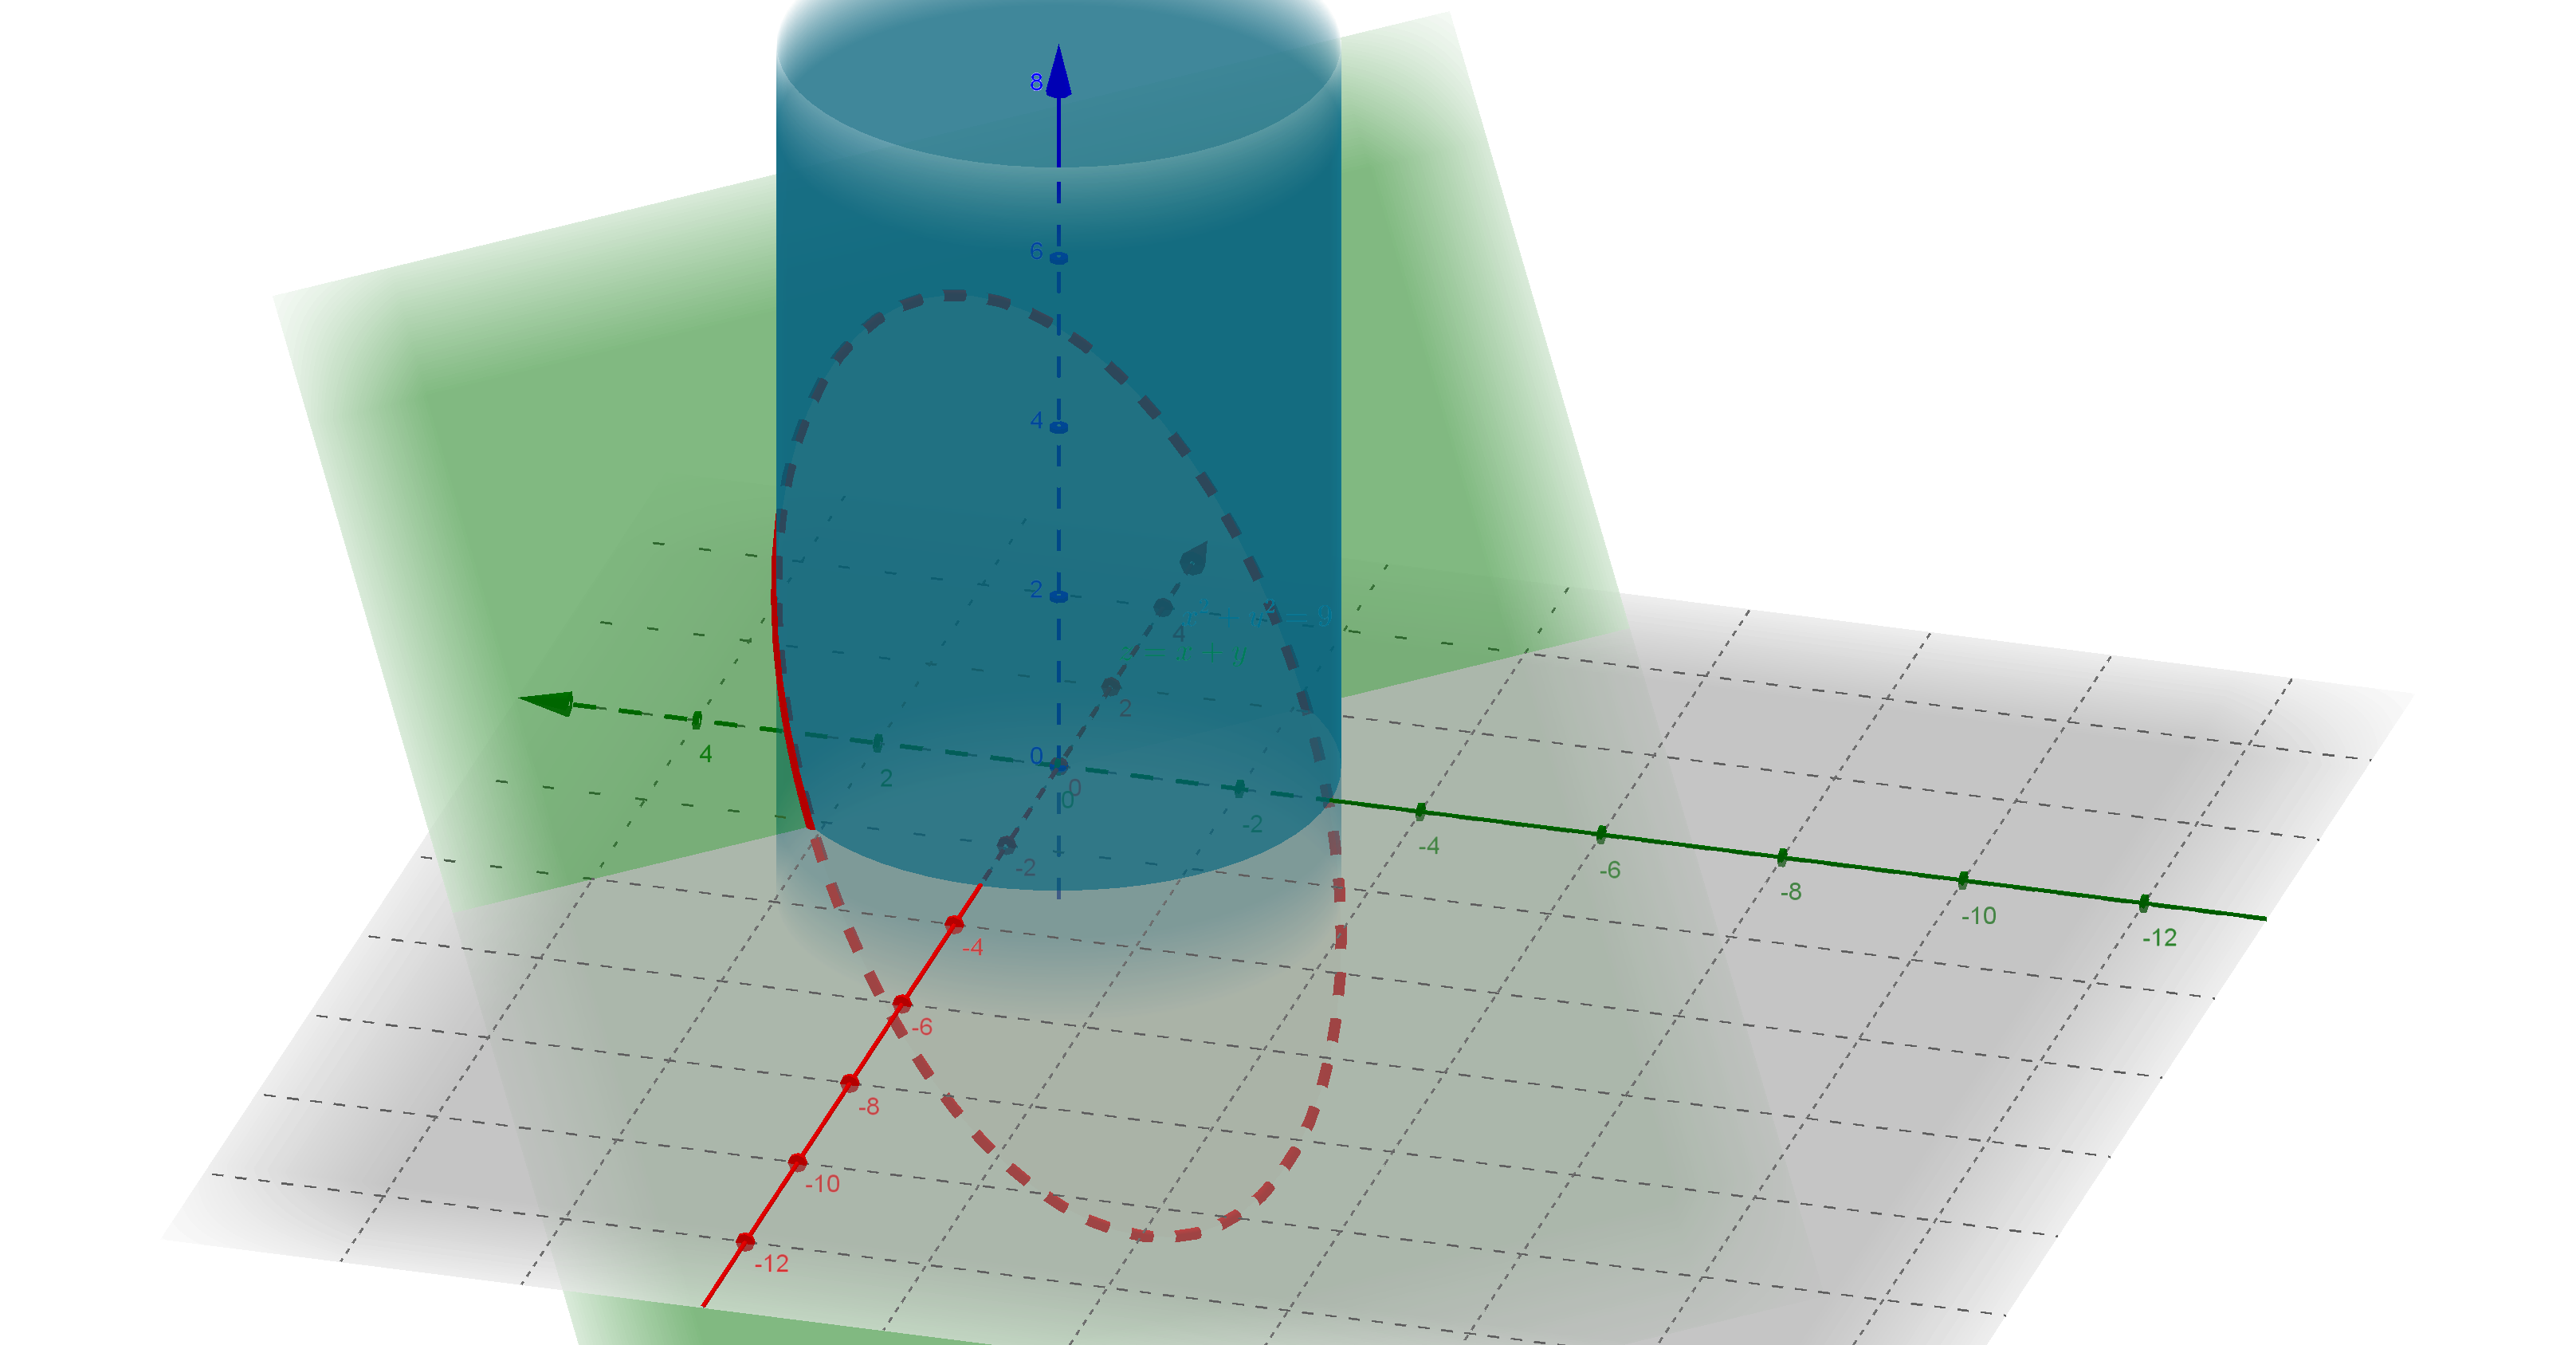
\includegraphics[scale=0.4]{p2b}
\end{center}
Se puede ver en color rojo la intersecci�n de las superficies.
\clearpage
\item[$c)$] Para realizar la parametrizacion podemos realizarlo de la siguiente manera:
$$x^2+y^2=9$$
Podemos ver que es un cilindro de radio 3 centrado en (0,0), podemos determinar los valores de $x$ y $y$ en terminos de un parametro $t$ de la siguiente manera:
\begin{align*}
x=&r\cos(t)+h\\
y=&r\sen(t)+k
\end{align*}
De acuerdo con eso tenemos:
\begin{align*}
x=&3\cos(t)\\
y=&3\sen(t)
\end{align*}
Con eso podemos averiguar $z$ en t�rminos de $t$
\begin{align*}
z&=x+y\\
z&=3\cos(t)+3\sen(t)
\end{align*}

Por lo que obtenemos la parametrizacion en t�rminos de $t$
$$\left\{\begin{matrix}
x =& 3\cos(t)& \\ 
y =& 3\sen(t)&t\in[0,2\pi] \\ 
z =& 3\cos(t) + 3\sen(t)&
\end{matrix}\right.$$
Y podemos ver como es ingresado en Geogebra:
\begin{center}
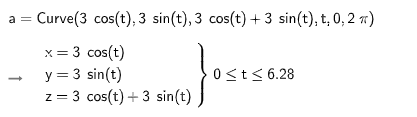
\includegraphics[scale=1]{c}
\end{center}
\begin{center}
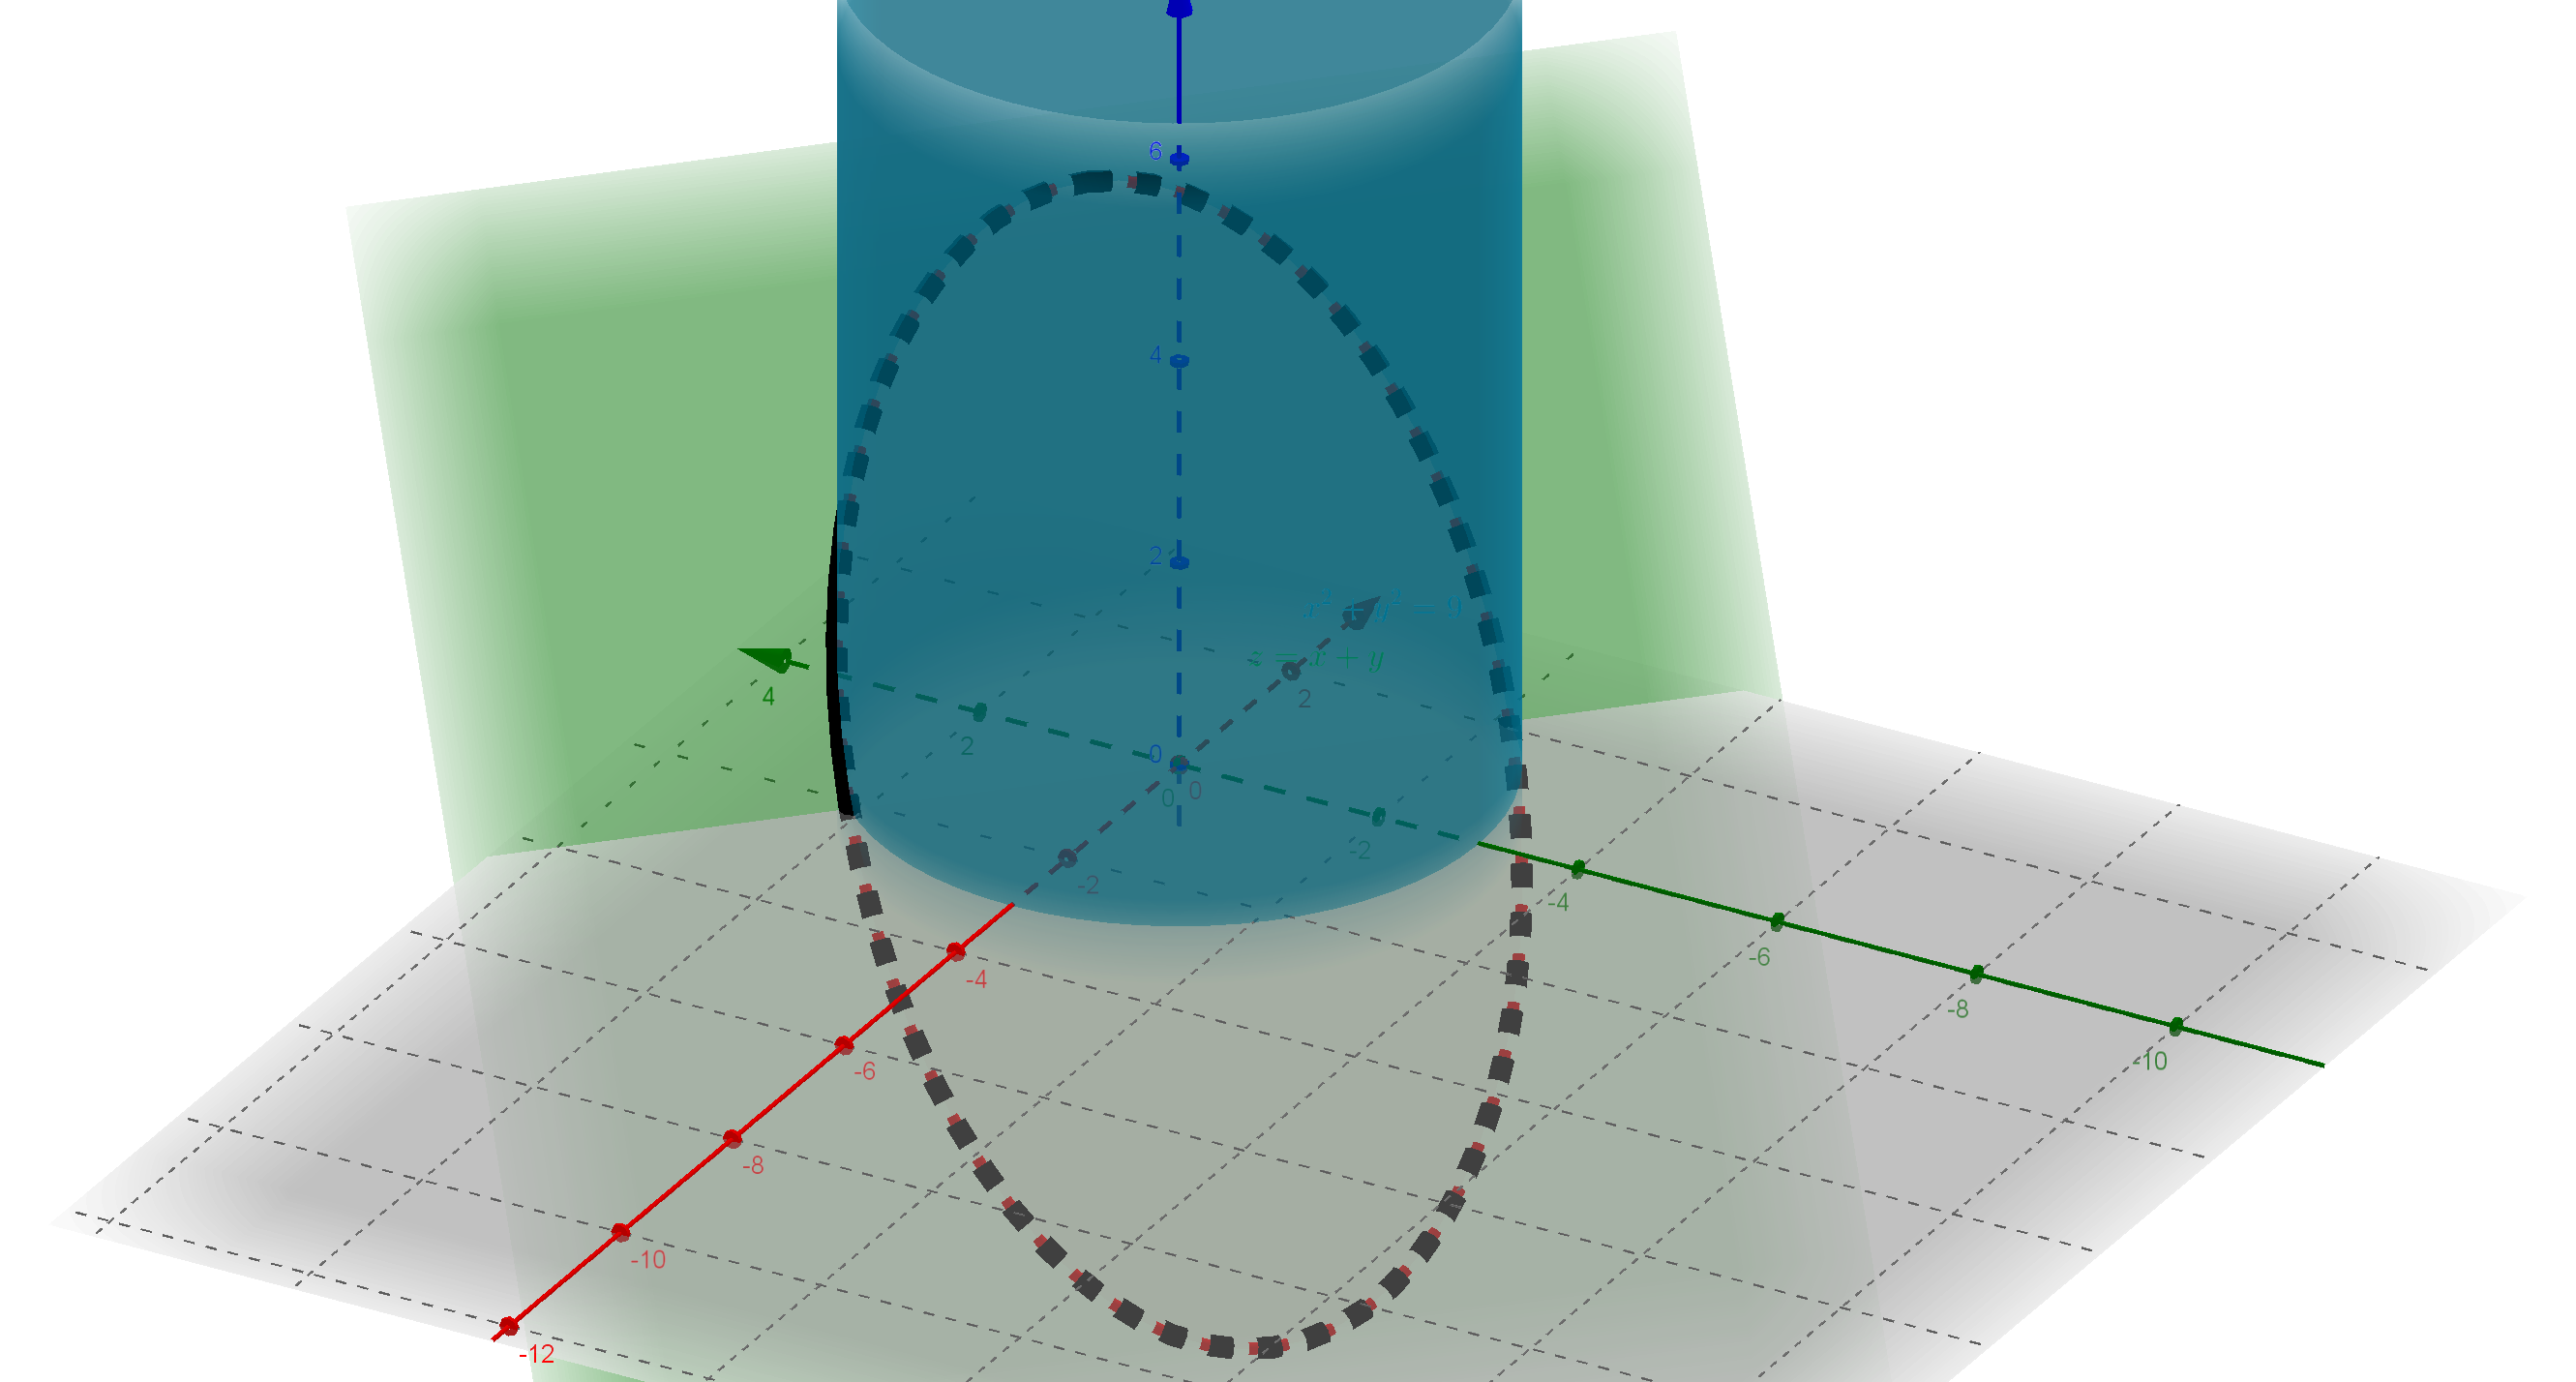
\includegraphics[scale=0.4]{p2c}
\end{center}
Se puede ver en color rojo la intersecci�n de las superficies y en negro la parametrizacion deducida.
\end{enumerate}
\clearpage
\section*{Pregunta 3}
\begin{enumerate}
\item[$a)$] Graficar mediante GeoGebra las superficies:
\begin{align*}
&x^2+y^2=1\\
&4z=x^2-y^2
\end{align*}
\begin{center}
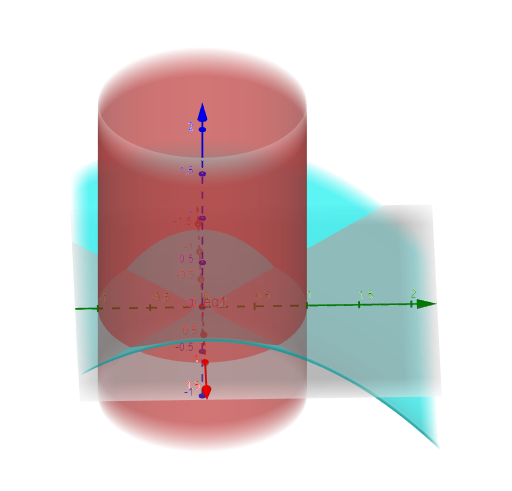
\includegraphics[scale=0.5]{p3a}
\end{center}
Se puede ver la silla esta en color celeste y el cilindro en rojo.

\item[$b)$] La intersecci�n .
\begin{center}
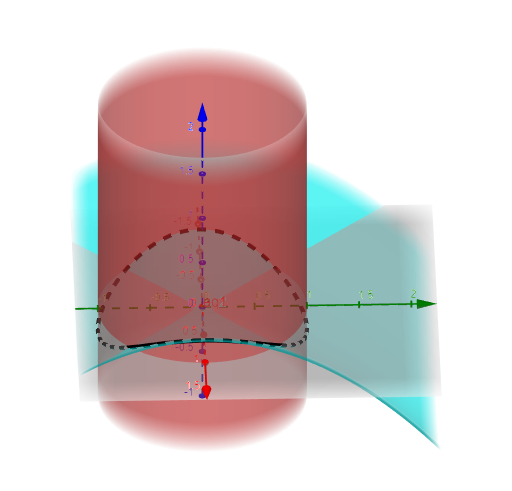
\includegraphics[scale=0.4]{p3cc}
\end{center}

\clearpage
\item[$c)$] Para realizar la parametrizacion podemos realizarlo de la siguiente manera:
$$x^2+y^2=9$$
Podemos ver que es un cilindro de radio 1 centrado en (0,0), podemos determinar los valores de $x$ y $y$ en terminos de un parametro $t$ de la siguiente manera:
\begin{align*}
x=&r\cos(t)+h\\
y=&r\sen(t)+k
\end{align*}
De acuerdo con eso tenemos:
\begin{align*}
x=&\cos(t)\\
y=&\sen(t)
\end{align*}
Con eso podemos averiguar $z$ en t�rminos de $t$
\begin{align*}
4z&=x^2+y^2\\
4z&=\cos^2(t)-\sen^2(t)\\
z=&= \frac{\cos^2(t)-\sen^2(t)}{4}\\
z=&= \frac{\cos(2t)}{4}
\end{align*}

Por lo que obtenemos la parametrizacion en t�rminos de $t$
$$\left\{\begin{matrix}
x =& \cos(t)& \\ 
y =& \sen(t)&t\in[0,2\pi] \\ 
z =& \frac{\cos(2t)}{4}&
\end{matrix}\right.$$
Y podemos ver como es ingresado en Geogebra , en color negro la intersecci�n de las superficies.
\begin{center}
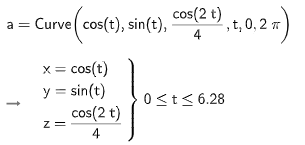
\includegraphics[scale=0.5]{p3c}
\end{center}
\begin{center}
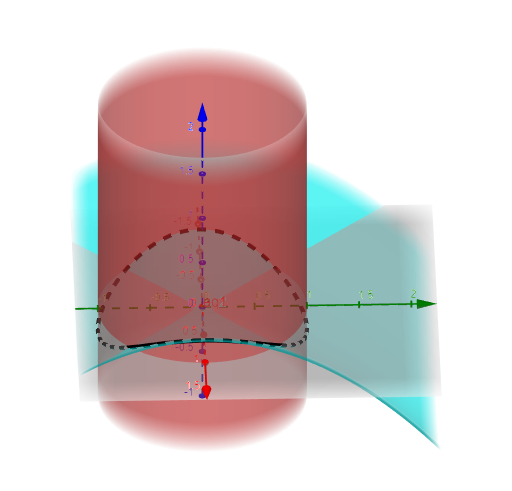
\includegraphics[scale=0.4]{p3cc}
\end{center}
\end{enumerate}
\end{document}